\section{Versuchsaufbau und Methodik}
\label{chap:methodik}

Zur Charakterisierung der Messstromwandler wurde ein Hochstrom-Prüfstand eingesetzt, der primäre Wechselströme von bis zu \SI{6000}{A} generieren kann.
Dies ermöglicht die Analyse der magnetischen Eigenschaften sowie der Messgenauigkeit unter realitätsnahen Betriebsbedingungen.
Das methodische Vorgehen untergliedert sich in die technische Beschreibung der Basiskomponenten, die kritische Analyse des ursprünglichen Messkonzepts sowie die daraus resultierende Systemoptimierung für die finalen Messreihen.

\subsection{Hochstrom-Prüfstand}
\label{sec:hochstrom_pruefstand}

Der Hochstrom-Prüfstand dient der Erzeugung und Regelung hoher Wechselströme für thermische und elektrodynamische Untersuchungen an elektrischen Betriebsmitteln.
Als Prüflinge fungieren in der Regel Niederspannungsschaltanlagen oder deren Teilkomponenten, die unter Lastbedingungen auf ihre thermische Belastbarkeit geprüft werden.
Die Anlage ermöglicht die Bereitstellung von Strömen bis \SI{6000}{A} bei einer geringen Sekundärspannung.

\subsubsection{Aufbau und Funktionsweise}
\label{sec:aufbau_funktionsweise}

Der Leistungspfad beginnt primärseitig mit einem motorbetriebenen Säulenstelltransformator der Firma Ruhstrat, der mit einer Leistung von \SI{90}{kVA} als zentrales Stellglied fungiert.
Dem Transformator sind Netzdrosseln nachgeschaltet, die zur Entkopplung von Stromspitzen dienen.
Die Spannungsstellung erfolgt stufenlos über verstellbare Kohlerollbürsten, wodurch eine variable Ausgangsspannung zwischen \SI{0}{V} und \SI{380}{V} bereitgestellt wird.
Diese Spannung speist den nachgeschalteten Hochstrom-Festtransformator von Rolf Janssen (Typ UI 260/420 M).
Mit einer Nennleistung von \SI{30}{kVA} transformiert dieser die Spannung auf eine Kleinspannung von \SI{6}{V} herab, was sekundärseitig die Realisierung von Prüfströmen bis zu \SI{6000}{A} am dreiphasigen Abgang ermöglicht.

\begin{figure}[H]
    \centering
    \includegraphics[width=0.8\textwidth]{03_Ressourcen/zeichnungen/aufbau_hochstrom_pruefstand.drawio.pdf}
    \caption{Blockschaltbild des Hochstrom-Prüfstandes mit Leistungs- und Signalpfaden}
    \label{pic:aufbau_hochstrom_pruefstand}
\end{figure}

\subsubsection{Regelungskonzept}
\label{sec:regelungskonzept}

Die Stromregelung ist als digitaler \gls{pid}-Regelkreis innerhalb der Siemens \gls{et200s} realisiert.
Der Anwender gibt über die \gls{wincc}-Visualisierung den gewünschten Sollstrom vor, welchen die \gls{sps} kontinuierlich mit dem rückgeführten Istwert vergleicht.
Als Stellgröße generiert die Steuerung Schaltbefehle für den Antriebsmotor des Säulenstelltransformators.
Um permanentes Nachregeln zu minimieren, die starke Stromspitzen erzeugen, ist eine Hysterese als Totband in den Regelalgorithmus integriert.
Die Visualisierung übernimmt dabei neben der Parametrierung auch das lückenlose Datenlogging der Versuchsverläufe.
Eine detaillierte Spezifikation der einzelnen Komponenten ist in Tabelle~\ref{tab:komponenten_hochstrom} zusammengefasst.
\begin{table}[H]
    \centering
    \caption{Detaillierte Spezifikation der Komponenten}
    \label{tab:komponenten_hochstrom}
    \small
    \begin{tabular}{@{}l l l l l@{}}
        \toprule
        \textbf{Komponente}      & \textbf{Typ}            & \textbf{Leistung / Bürde}

                                 & \textbf{Primär / Input} & \textbf{Sekundär / Output}                                                                                \\ \midrule
        Säulenstelltransformator & Ruhstrat                & \SI{90}{kVA}

                                 & \SI{380}{V}             & \SI{0}{V}--\SI{380}{V} (\SI{70}{A})                                                                       \\
        Festtransformator        & Janssen                 & \SI{30}{kVA}

                                 & \SI{380}{V}             & \SI{6}{V} (\SI{5000}{A})                                                                                  \\
        Stromwandler             & Celsa ICG               & \SI{5}{VA}

                                 & \SI{6000}{A}            & \SI{5}{A} (Kl. 0,2S)                                                                                      \\
        
        Messumformer (K-3)       & 3-K Elektrik            & --                                                                          & \SI{0}{A}--\SI{5}{A} AC & 
        \SI{0}{mA}--\SI{20}{mA} \gls{dc}                                                                                                                               \\ \midrule
        \textbf{Leittechnik}     & \textbf{Typ}            & \multicolumn{3}{l}{\textbf{Beschreibung}}

        \\ \cmidrule(r){1-2}
        Steuerung                & Siemens \gls{et200s}    & \multicolumn{3}{l}{\gls{profinet}-Anbindung, Stromregelung, Analogeingänge}

        \\
        Visualisierung           & Siemens \gls{wincc}     & \multicolumn{3}{l}{\gls{hmi}-System, Prozessüberwachung, Datenlogging}

        \\ \bottomrule
    \end{tabular}
\end{table}


\subsubsection{Ursprünglicher Aufbau der Messstrecke}
\label{sec:aufbau_alter_messstrecke}

\begin{figure}[H]
    \centering
    \includegraphics[width=0.8\textwidth]{03_Ressourcen/zeichnungen/aufbau_messstrecke.drawio.pdf}
    \caption{Schematischer Aufbau der Messstrecke zur Ermittlung der Messabweichung}
    \label{pic:aufbau_messstrecke}
\end{figure}

Der erste Aufbau der Messstrecke (siehe Abbildung \ref{pic:aufbau_messstrecke}) sah zwei parallele Erfassungspfade vor.
Zur Bestimmung des Referenzwertes der Einspeisung wurden die K-3-Messumformer genutzt, welche das Signal an die \gls{sps} übermittelten.
Parallel dazu wurde das Ausgangssignal des Prüflings mit einem Digitalmultimeter von Fluke im Modus „Acquire“ erfasst.
%Die Inbetriebnahme diente dazu, die Funktionalität der Regelung sowie die Genauigkeit der Messwerterfassung unter Lastbedingungen zu verifizieren.

\subsubsection{Schwachstellen im Messkonzept}
\label{sec:fehleranalyse}

Die Auswertung der ersten Messreihen zeigt Abweichungen, die über den gesamten Messbereich auftreten.
In Abbildung \ref{pic:dia_messstrecke_alt} sind die Verläufe der Messumformer K-3 (blau) und der Rogowskispulen (orange) dargestellt.
Die Rogowskispulen wurden parallel eingesetzt, um deren Eignung für die Prüfung der Wandler zu untersuchen.
Beide Systeme erfassten die Messwerte zeitgleich an einem Messpunkt hinter dem Festtransformator.
Als Referenz dient die Genauigkeitsklasse 0,2, da die primärseitigen Stromwandler der Klasse 0,2S entsprechen.
Die grafische Darstellung verdeutlicht, dass beide Messsysteme die durch die Norm vorgegebenen Toleranzgrenzen (gestrichelte Linien) nicht einhalten.
In Phase L1 überschreitet der Messumformer K-3 ab einer Last von 50\,\% den positiven Grenzwert, während die Rogowskispulen eine negative Abweichung zwischen -1\,\% und -2,5\,\% aufweisen.
In Phase L2 zeigt der Messumformer K-3 bei 20\,\% Last einen Abfall der Genauigkeit auf circa -2\,\%, wohingegen die Rogowskispulen eine positive Abweichung von über 1\,\% erreichen.
Da die Verläufe der beiden Messsysteme voneinander abweichen, kann kein eindeutiger Referenzwert für den Primärstrom bestimmt werden.

\begin{figure}[H]
    \centering
    \includegraphics[width=0.8\textwidth]{03_Ressourcen/diagramme/dia_messstrecke_alt/dia_messstrecke_alt-Zusammenfassung_MultiCurrent.pdf}
    \caption{Analyse der Messabweichung und Standardabweichung der Phasen L1, L2 und L3 im ursprünglichen Versuchsaufbau}
    \label{pic:dia_messstrecke_alt}
\end{figure}


Die im unteren Teil der Abbildung \ref{pic:dia_messstrecke_alt} dargestellte Standardabweichung zeigt, dass beide Messgeräte im niedrigen Strombereich eine erhöhte Varianz aufweisen.
Dies ist darauf zurückzuführen, dass der Säulenstelltransformator bei geringen Strömen einen begrenzten Stellbereich besitzt, woraus eine geringere Stabilität des Stromwertes resultiert aus der Regelung.
Mit zunehmender Stromstärke reduziert sich dieses Rauschen im Messsignal. Dabei weisen die K-3-Messumformer eine geringere Schwankungsbreite auf als die Rogowskispulen.
Aufgrund dieser Ergebnisse sind beide Messverfahren für eine Referenzmessung im Rahmen der Genauigkeitsprüfung unzureichend.
Im folgenden Abschnitt \ref{sec:optimierung} wird die Systemoptimierung erläutert, um eine präzisere Messwerterfassung zu realisieren.

\subsection{Optimiertes Messsystem}
\label{sec:optimierung}

Wie im vorangegangenen Abschnitt dargelegt, erfüllte die ursprüngliche Messstrecke nicht die Anforderungen an eine präzise Genauigkeitsprüfung von Messstromwandlern.
Aus diesem Grund wurde eine Optimierung des Hochstrom-Prüfstandes durchgeführt. Das primäre Ziel dieser Maßnahmen war die Steigerung der Messgenauigkeit sowie die Automatisierung des Prüfablaufs, um reproduzierbare und direkt vergleichbare Ergebnisse sicherzustellen.
Zur technischen Umsetzung wurden zwei digitale Energiemessgeräte der Siemens-Produktfamilie ausgewählt.
Das Modell PAC3220, welches für die Erfassung des Prüflingsstroms eingesetzt wird \cite[S.~97]{siemens_pac3220_2019}, sowie das zur Überwachung der Einspeisung genutzte PAC4220 \cite[S.~94]{siemens_pac4220_2024} verfügen jeweils über die Genauigkeitsklasse 0,2 für die Strommessung.
Diese Geräte ermöglichen durch optionale Erweiterungsmodule eine direkte Integration in die Systemumgebung der Siemens \gls{et200s} via \gls{profinet}-Protokoll.
Ein wesentlicher Vorteil dieser Konfiguration liegt in der dezentralen Messwerterfassung unmittelbar am Messpunkt.
Dadurch lassen sich parasitäre Effekte über lange Messleitungen minimieren. Die Einbindung in die \gls{sps} erfolgt durch eine direkte zyklische Datenübertragung, wodurch die manuelle Abfrage von Registern entfällt und eine zeitsynchrone Datenbasis für beide Messpunkte geschaffen wird.

\begin{figure}[H]
    \centering
    \includegraphics[width=0.8\textwidth]{03_Ressourcen/zeichnungen/aufbau_hochstrom_pruefstand_new.drawio.pdf}
    \caption{Schematischer Aufbau der optimierten Messstrecke mit Siemens SENTRON Messgeräten}
    \label{pic:aufbau_messstrecke_neu}
\end{figure}

Die in Abbildung \ref{pic:aufbau_messstrecke_neu} dargestellte Systemarchitektur verdeutlicht die informationstechnische Vernetzung des optimierten Messaufbaus.
Während der obere Teil des Schemas den bereits beschriebenen Leistungspfad darstellt, erfolgt die messtechnische Erfassung der Primärströme zyklisch durch die Geräte PAC 4220 (Einspeisung) und PAC 3220 (Prüfling).
Die erfassten Stromwerte werden in \gls{wincc} archiviert und stehen dort für die Prozessüberwachung zur Verfügung.
Über die Benutzeroberfläche (\gls{hmi}) können diese Daten als \gls{csv}-Datei exportiert werden.
Diese Datei dient als Grundlage für die anschließende Genauigkeitsmessung und die Auswertung der Versuchsreihen.

\subsubsection{Systemintegration und Programmentwicklung}
\label{sec:integration_programmierung}

Die technische Umsetzung des optimierten Messsystems umfasst sowohl die informationstechnische Einbindung der Hardware-Komponenten als auch die Entwicklung der steuerungstechnischen Ablauflogik.
Zur Adressierung der SENTRON-Messgeräte wird jedem Gerät in der Hardware-Konfiguration des Simatic Managers ein eindeutiger Gerätename sowie eine IP-Adresse zugewiesen.
Diese Zuweisung ist notwendig, um die Kommunikation der Teilnehmer innerhalb des \gls{profinet}-Netzwerks mit der \gls{sps} zu ermöglichen.
Innerhalb des Hardware-Konfigurators werden die spezifischen Messwerte der Geräte auf die Eingangsadressen der \gls{sps} abgebildet.
Die so bereitgestellten Rohwerte werden im Anwenderprogramm der Steuerung aus dem Peripheriebereich ausgelesen und in \gls{db}s übertragen.
Für die Erfassung der Daten in \gls{wincc} wird im Variablenhaushalt des Visualisierungssystems eine Kommunikationsverbindung zur Steuerung projektiert.
Die Variablen für die gemessenen Ströme werden direkt mit den entsprechenden Speicheradressen innerhalb der \gls{db}s verknüpft.
Über diese Verbindung werden die Werte der Ströme in regelmäßigen Abständen vom System ausgelesen, auf dem \gls{hmi} angezeigt und für den späteren Export als \gls{csv}-Datei in der Datenbank gespeichert.
Die Automatisierung des Prüfablaufs wird über die \gls{sps} realisiert, wobei der vorhandene \gls{pid}-Regler zur präzisen Stromeinstellung genutzt wird.
Für die Genauigkeitsmessung eines Wandlers sind gemäß Norm primär die Prüfpunkte bei 5~\%, 20~\%, 100~\% und 120~\% des Primär-Nennstroms von Bedeutung.
Um eine detailliertere Kennlinie zu erhalten und das Verhalten des Wandlers umfassender zu charakterisieren, wurden dem Prüfablauf weitere Messpunkte hinzugefügt.
Die automatisierte Erfassung umfasst somit die Pegel 5~\%, 20~\%, 50~\%, 80~\%, 90~\%, 100~\% und 120~\%.
Um diese Messpunkte automatisiert anzufahren, wurde eine Schrittkette entwickelt. Diese durchläuft die Prüfpegel sequenziell und hält jeden Messpunkt für eine Dauer von fünf Minuten konstant.
Dieser Zeitraum gewährleistet eine ausreichende thermische Sättigung des Wandlerkerns und ermöglicht eine valide Mittelwertbildung der Messdaten.

\begin{figure}[H]
    \centering
    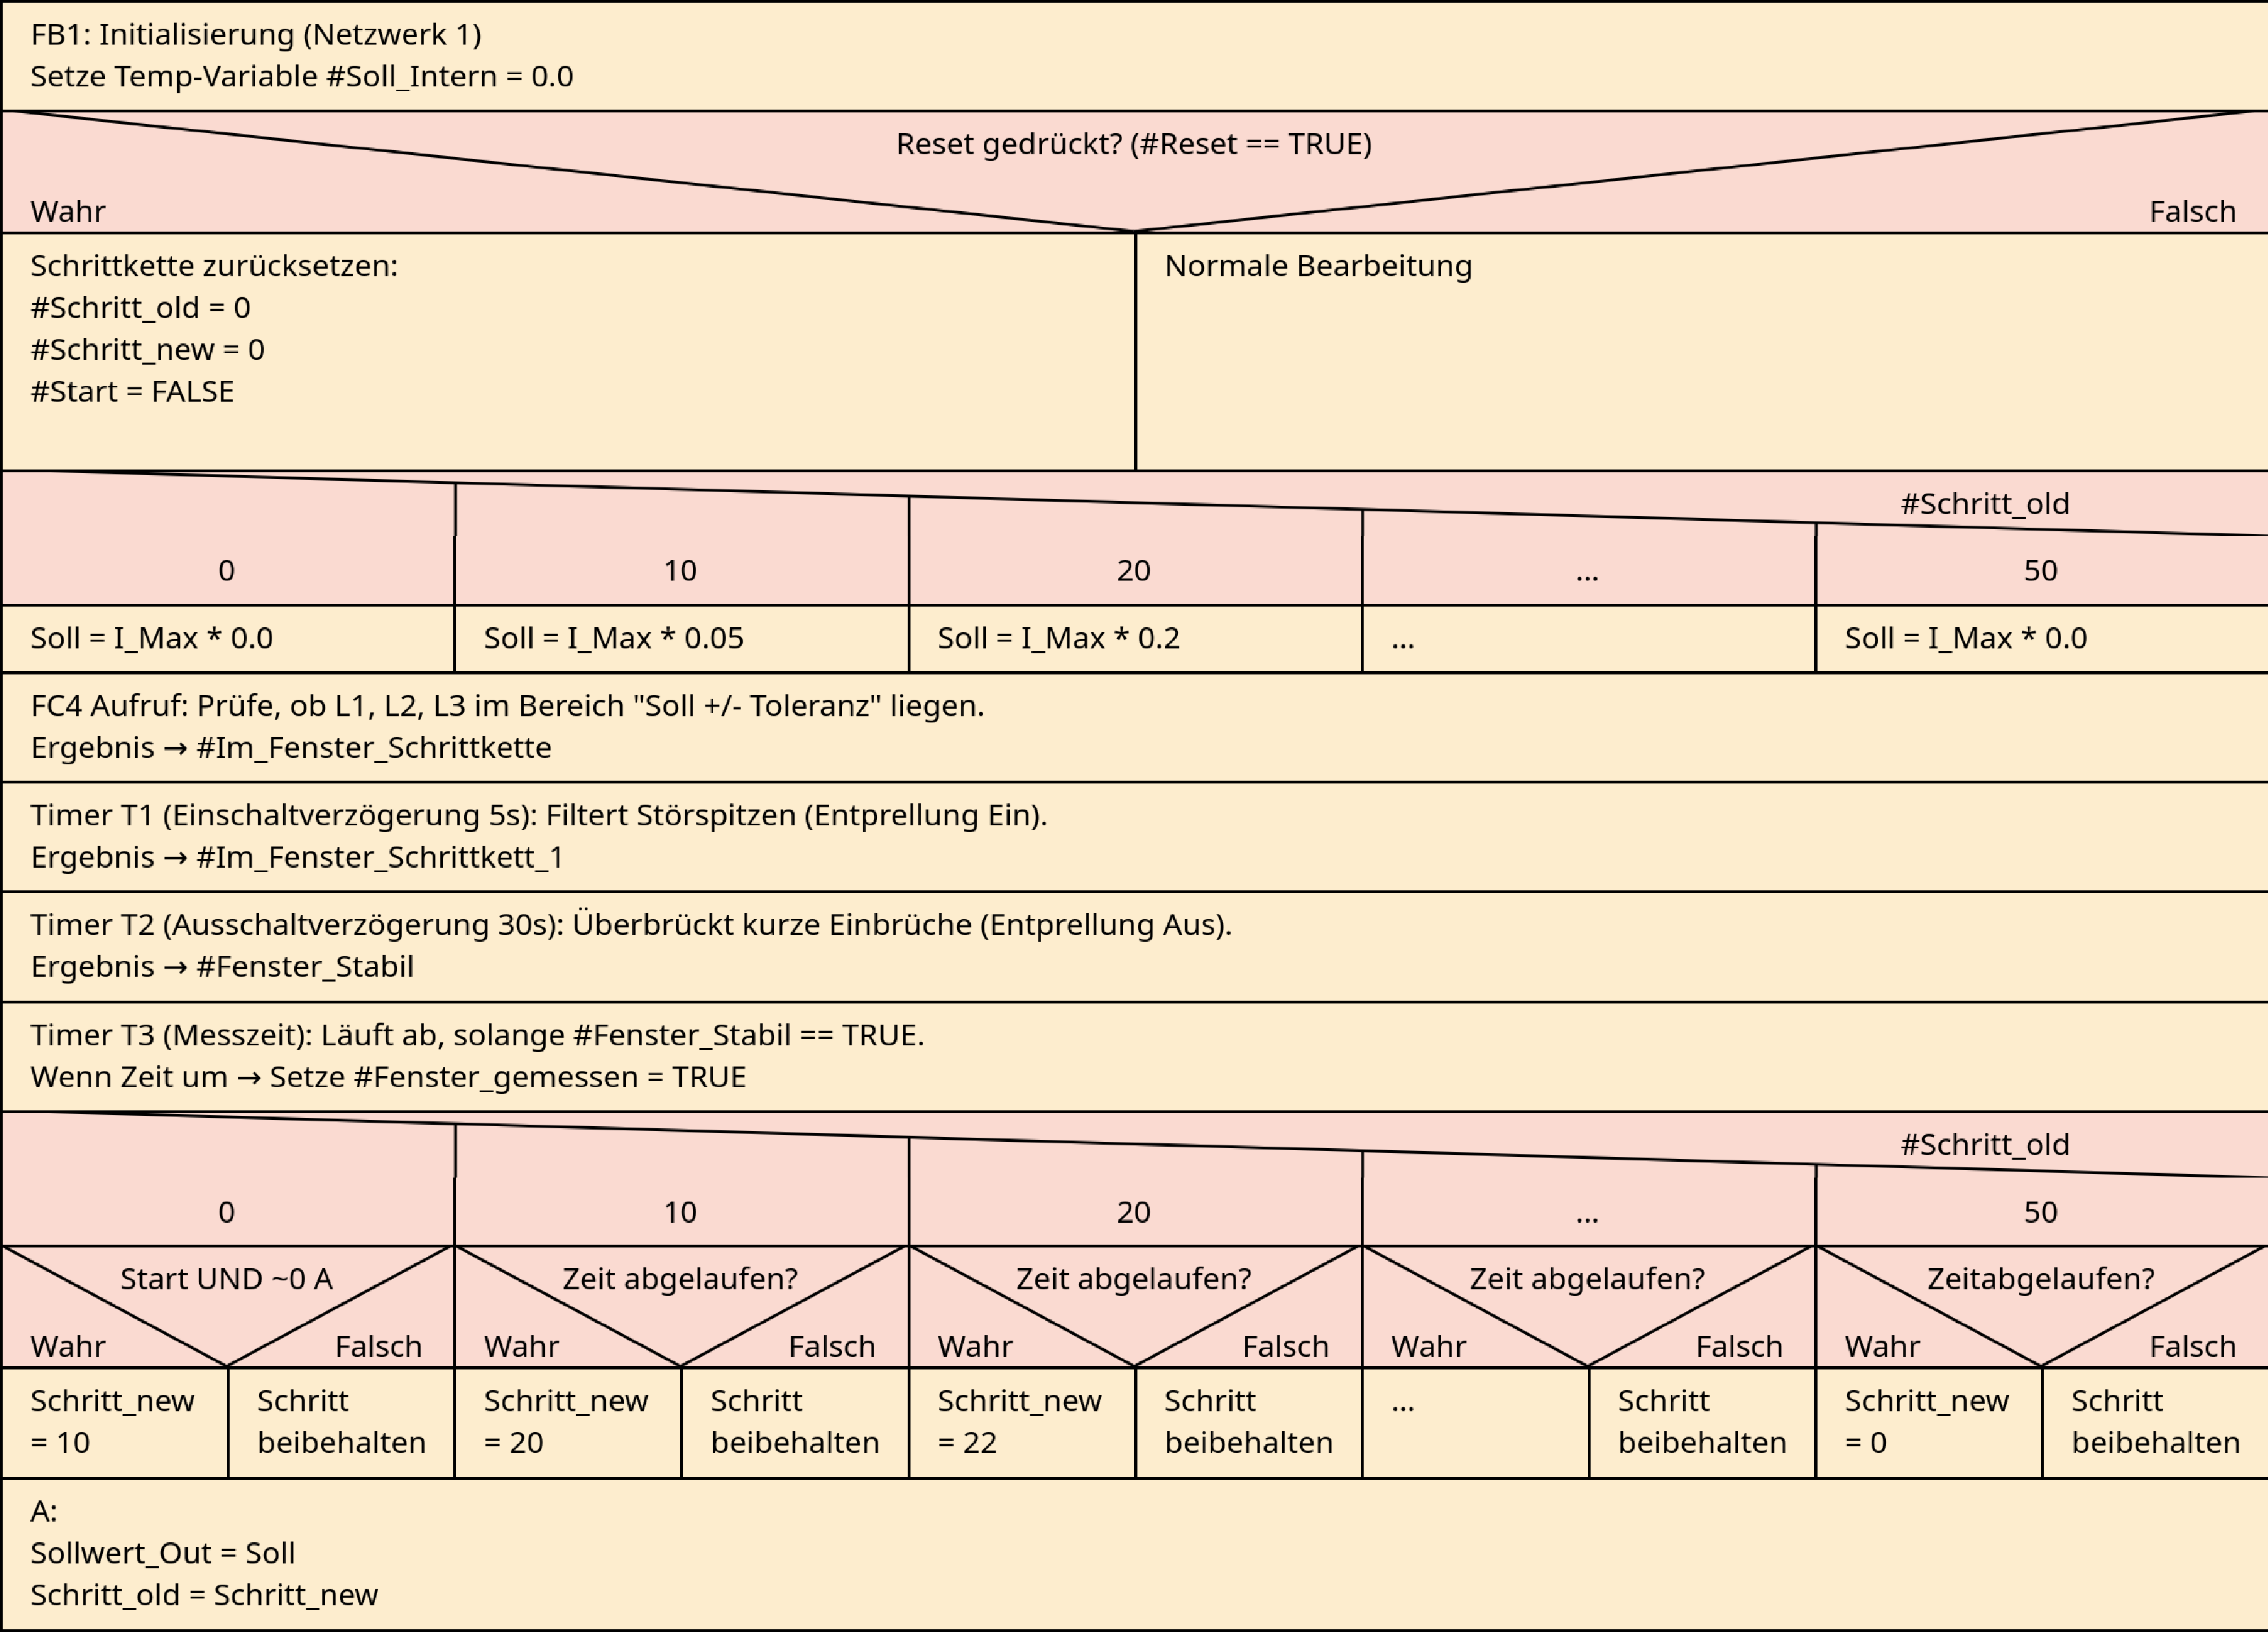
\includegraphics[width=0.8\textwidth]{03_Ressourcen/pdf/step7_programm/strukto_fb1.pdf}
    \caption{Struktogramm der Schrittkette zur automatisierten Kennlinienaufnahme (\gls{fb}1)}
    \label{pic:strukto_fb1}
\end{figure}

Der logische Ablauf dieser Automatisierung ist im Struktogramm des Funktionsbausteins \gls{fb}1 dargestellt.
Der Baustein übernimmt die zentrale Steuerung, wobei zu Beginn eine Initialisierung erfolgt, bei der die interne Sollwert-Variable auf Null gesetzt wird.
Im Falle eines aktiven Reset-Signals wird die gesamte Schrittkette zurückgesetzt, indem die Schrittzähler auf Null und das Startsignal auf den Zustand Falsch gesetzt werden.
Während der normalen Bearbeitung wird basierend auf dem aktuellen Schrittwert der entsprechende Sollwert für den Primärstrom vorgegeben.
So entspricht beispielsweise Schritt 10 einer Last von 5~\% und Schritt 20 einer Last von 20~\% des Maximalstroms.
Zur Überprüfung der Messwertstabilität wird die Funktion \gls{fc}4 aufgerufen, welche kontrolliert, ob die Phasenströme innerhalb eines definierten Toleranzfensters um den Sollwert liegen.
Ein Zeitglied T1 dient dabei der Entprellung beim Eintritt in das Fenster, während das Zeitglied T2 kurze Einbrüche überbrückt, um eine stabile Datenbasis sicherzustellen.
Die eigentliche Messzeit wird durch den Timer T3 gesteuert, der nach Ablauf die Messung am aktuellen Punkt als abgeschlossen markiert.
Die Weiterschaltlogik der Schrittkette wertet diesen Status aus: Im Ausgangszustand wird auf die Startbedingungen gewartet, während in den aktiven Prüfschritten der Übergang zum nächsten Pegel erst nach erfolgreichem Ablauf der Messzeit erfolgt.
Abschließend werden der ermittelte Sollwert an den Regler ausgegeben und der Schrittstatus für den nächsten Zyklus aktualisiert.

\subsubsection{Softwaregestützte Prozesskette zur Datenauswertung}
\label{sec:datenaufbereitung_analyse}

Die von der Visualisierung exportierten Rohdaten liegen im \gls{csv}-Format vor und enthalten die zeitlichen Verläufe der Ströme $I_{prim}$ (Referenz) und $I_{sek}$ (Prüfling).
Angesichts des Umfangs der Untersuchung, die 31 Konfigurationen mit jeweils zwei Messgeräten und drei Phasen umfasst, ergaben sich insgesamt über 180 auszuwertende Einzelmessreihen.
Eine manuelle Verarbeitung dieser Datenmenge mittels Tabellenkalkulation wäre zeitaufwendig und anfällig für Übertragungsfehler gewesen.
Aus diesem Grund wurde eine mehrstufige Pipeline in der Programmiersprache Python entwickelt (unter Nutzung der Bibliothek \textit{pandas}), welche den Auswertungsprozess von der Rohdatenfilterung bis zur grafischen Darstellung automatisiert.
Da die Schrittkette (siehe Abschnitt \ref{sec:integration_programmierung}) physikalisch bedingte Einschwingvorgänge beim Anfahren der Lastpunkte aufweist, ist zunächst eine Filterung der Rohdaten erforderlich.
Ziel ist es, die stabilen Bereiche für die Genauigkeitsberechnung heranzuziehen. Zur Organisation wurde hierfür der \textit{Messdaten-Selektor} (Skript: \texttt{messdaten\_selektor.py}) entwickelt.
Diese Software visualisiert die Zeitverläufe der Messungen und ermöglicht eine interaktive Bearbeitung.
Der Anwender prüft visuell die Kennlinien und definiert manuell die zeitlichen Grenzen (Start- und Endzeitpunkt) der stabilen Lastplateaus über eine Eingabemaske.

\begin{figure}[H]
    \centering
    \includegraphics[width=0.8\textwidth]{03_Ressourcen/pdf/manueller_rohdaten_export/gesamtansicht.png}
    \caption{Benutzeroberfläche des manuellen Messdaten-Selektors}
    \label{pic:manual_tagger}
\end{figure}

Dies dient der Datenzuverlässigkeit, da instabile Randbereiche ausgeschlossen werden.
Auf Basis dieser Benutzereingaben werden die definierten Bereiche extrahiert und in separate, sortierte \gls{csv}-Dateien für jede Messung überführt.
Dieser Schritt der Segmentierung verringert den Zeitaufwand in der weiteren Verarbeitung und stellt eine einheitliche Datenbasis sicher.
Um die segmentierten Messreihen vergleichbar zu machen, erfolgt im Anschluss die mathematische Weiterverarbeitung durch den \textit{Daten-Aggregator} (Skript: \texttt{daten\_aggregator.py}).
Dieses Modul durchläuft automatisiert die sortierten Dateien und führt die statistischen Berechnungen durch.
Dabei werden für jede Messreihe verschiedene Vergleichsoperationen durchgeführt, um die Güte der Versuchsführung sowie die Genauigkeit des Prüflings zu bewerten.
Tabelle~\ref{tab:berechnungsmodi} gibt eine Übersicht über die implementierten Berechnungsmodi und deren Zielsetzung.

\begin{table}[H]
    \centering
    \caption{Übersicht der Berechnungsmodi im Daten-Aggregator}
    \label{tab:berechnungsmodi}
    \renewcommand{\arraystretch}{1.2}
    \begin{tabular}{@{}l l l p{5cm}@{}}
        \toprule
        \textbf{Modus} & \textbf{Referenzwert ($I_{ref}$)} & \textbf{Messwert ($I_{ist}$)} & \textbf{Untersuchungsziel} \\ \midrule
        Regelgüte & Nennstrom ($I_{soll}$) & Einspeisung ($I_{prim}$) & Überprüfung, ob der Prüfstand den geforderten Arbeitspunkt eingeregelt hat. \\ \addlinespace
        Nennwert-Fehler & Nennstrom ($I_{soll}$) & Prüfling ($I_{sek}$) & Abweichung des Wandlers vom theoretischen Sollwert (inkl. Regelabweichung). \\ \addlinespace
        Wandler-Fehler & Einspeisung ($I_{prim}$) & Prüfling ($I_{sek}$) & \textbf{Messabweichung} des Prüflings relativ zur Referenzmessung (Klasse 0,2S). \\ \bottomrule
    \end{tabular}
\end{table}

Die Berechnung der prozentualen Messabweichung $\varepsilon$ erfolgt analog zu den in Abschnitt \ref{sec:messabweichung_fehlerfortpflanzung} (Gleichung \ref{eq:messabweichung_epsilon}) dargelegten Grundlagen. Für die automatisierte Auswertung wird folgende Berechnungsvorschrift angewendet:

\begin{equation}
    \label{eq:messabweichung_allg}
    \varepsilon = \frac{I_{ist} - I_{ref}}{I_{ref}} \cdot 100\,\%
\end{equation}

Hierbei beschreibt $I_{ist}$ den arithmetischen Mittelwert der gemessenen Stromstärke des Prüflings über das stabile Zeitfenster, während $I_{ref}$ den entsprechenden Referenzwert darstellt.
Zusätzlich wird für jeden Lastpunkt die Standardabweichung $\sigma$ berechnet, um die Signalstabilität zu quantifizieren:

\begin{equation}
    \label{eq:standardabweichung}
    \sigma = \sqrt{\frac{1}{N-1} \sum_{i=1}^{N} (x_i - \bar{x})^2}
\end{equation}

Die resultierenden Datensätze, bestehend aus Mittelwerten ($\bar{x}$), Standardabweichungen ($\sigma$) und berechneten Fehlern ($\varepsilon$), werden abschließend in einer Datenbank im Apache-Parquet-Format (\texttt{messdaten\_db.parquet}) persistiert.
Dieses spaltenorientierte Speicherformat bietet gegenüber \gls{csv}-Dateien eine höhere Lese-Performance für die nachgelagerte Visualisierung.
Die grafische Aufbereitung der Ergebnisse erfolgt durch das \textit{Visualisierungs-Dashboard} (Skript: \texttt{visualisierungs\_dashboard.py}).
Da die rechenintensiven Vorarbeiten bereits durch die Aggregation abgeschlossen sind, greift dieses Tool auf die Datenbank zu.
Dies ermöglicht dem Anwender, über Filterfunktionen Diagramme zu erstellen. So können beispielsweise verschiedene Wandler übereinandergelegt oder der Einfluss der Leitergeometrie verglichen werden, ohne dass eine erneute Berechnung der Rohdaten erforderlich ist.


\subsubsection{Auswertung der neuen Messstrecke}
\label{sec:auswertung_messstrecke}

Die Validierung der optimierten Messstrecke belegt eine signifikante Steigerung der Messgüte im Vergleich zu den ursprünglichen Komponenten.
In Abbildung \ref{pic:dia_messstrecke_neu} ist der Fehlerverlauf des neu installierten Energiemessgerätes PAC 4220 (magenta) im direkten Vergleich zum Messumformer K-3 (blau) und den Rogowskispulen (orange) dargestellt.
Der magenta Kurvenverlauf verdeutlicht, dass das PAC 4220 über nahezu den gesamten Lastbereich innerhalb des normativen Toleranzbandes der Genauigkeitsklasse 0,2 verbleibt.
Ab einer Last von 20\,\% des Nennstroms stabilisiert sich die Messabweichung nahe der Nulllinie.
Lediglich im Bereich geringer Ströme (5\,\%) ist eine Abweichung außerhalb der Normgrenzen erkennbar.
Wie bereits in Abschnitt \ref{sec:fehleranalyse} analysiert, resultiert dieser Effekt aus dem begrenzten Stellbereich des Säulenstelltransformators, der bei minimaler Auslenkung keine stabile Stromvorgabe ermöglicht.
Durch die hohe Auflösung des PAC 4220 kann diese physikalische Grenze des Prüfstandes nun präzise messtechnisch erfasst werden.

\begin{figure}[H]
    \centering
    \includegraphics[width=1.0\textwidth]{03_Ressourcen/diagramme/dia_messstrecke_neu/dia_messstrecke_neu-Zusammenfassung_MultiCurrent.pdf}
    \caption{Vergleichende Analyse der Messabweichung (oben) und Standardabweichung (unten) unter Einsatz des PAC 4220}
    \label{pic:dia_messstrecke_neu}
\end{figure}


Die im unteren Teil der Abbildung \ref{pic:dia_messstrecke_neu} visualisierte Standardabweichung verdeutlicht die Präzision der Messsysteme bezüglich der Streuung.
Hierbei zeigt sich, dass das PAC 4220 und der Messumformer K-3 ein sehr ähnliches Verhalten mit einer vergleichbar geringen Streuung aufweisen.
Ab einer Last von 50\,\% sinkt die Standardabweichung für beide Geräte auf ein Niveau von unter 0,5\,\%.
Im Gegensatz dazu weisen die Rogowskispulen über den gesamten Messbereich eine deutlich höhere Streuung auf, was auf eine geringere Reproduzierbarkeit der Messwerte hindeutet.
Obwohl die K-3-Umformer eine ähnlich geringe Streuung wie das PAC-Messgerät erzielen, verbleiben sie aufgrund ihrer hohen systematischen Abweichung außerhalb der geforderten Genauigkeitsklasse.
Die Ergebnisse bestätigen somit, dass erst durch den Einsatz der digitalen PAC-Messgeräte eine valide Datenbasis geschaffen wurde, die sowohl eine geringe Streuung als auch eine normgerechte Genauigkeit für die Charakterisierung der Stromwandler vereint.

\subsection{Versuchsaufbau der Messobjekte und Leiteranordnung}
\label{sec:geometrie_kupferschienen}

Zusätzlich zur messtechnischen Optimierung wird die geometrische Anordnung des Primärleiters variiert, um deren Einfluss auf die Fremdfeldbeeinflussung zu untersuchen.

\subsubsection{Auswahl und Spezifikation der Messstromwandler}
\label{sec:auswahl_wandler}

Für die experimentellen Untersuchungen werden Stromwandler der Hersteller MBS, Celsa und Redur eingesetzt.
Die Auswahl deckt ein Spektrum von marktüblichen Standardwandlern bis hin zu spezialisierten Modellen mit integriertem Fremdfeldschutz ab.
Ziel dieser Zusammenstellung ist es, eine belastbare Datenbasis für die Analyse der Beeinflussungseffekte unter verschiedenen technologischen Voraussetzungen zu schaffen.
Tabelle \ref{tab:wandler_spezifikationen_erweitert} fasst die technischen Kenndaten der Prüflinge zusammen. Neben dem Nennstrom $I_n$ und der Bemessungsleistung $S_n$ ist das Gehäusevolumen aufgeführt.
Dieses dient als Vergleichsgröße für die Wirtschaftlichkeitsbetrachtung und errechnet sich aus dem Produkt der maximalen äußeren Gehäuseabmessungen (Höhe $\times$ Breite $\times$ Tiefe).
Es ist anzumerken, dass es sich hierbei um eine Vereinfachung handelt, die den Wandler auf seinen quaderförmigen Hüllkörper reduziert.
Spezifische Geometrien, wie etwa Verjüngungen oder Abrundungen am Gehäuse, werden in dieser Berechnung vernachlässigt, sodass das tatsächliche Materialvolumen geringer ausfallen kann.
Für die konstruktive Bewertung in Schaltanlagen ist diese Betrachtungsweise jedoch maßgeblich, da für die Montageplanung der maximale Platzbedarf (Bauraum) reserviert werden muss, den der Wandler im Anschlussraum effektiv beansprucht.
\begin{table}[H]
    \centering
    \caption{Erweiterte Spezifikationen und wirtschaftliche Kennwerte der Prüflinge}
    \label{tab:wandler_spezifikationen_erweitert}
    \begin{tabular}{@{}lll
            S[table-format=4.0]
            S[table-format=2.1]
            S[table-format=4.0]
            S@{}}
        \toprule
        \textbf{Hersteller}
                                                     & 
        \textbf{Typ}                                 & 
        \textbf{Technologie}                         & 
        {\textbf{$I_n$ [\si{\ampere}]}}
                                                     & 
        {\textbf{$S_n$ [\si{\volt\ampere}]}}         & 
        {\textbf{Volumen [\si{\centi\meter\cubed}]}} & 
        \textbf{Preis [\euro]}
        \\
        \midrule
        Celsa                                        & ALO 10030
                                                     & Standard      & 2000        & 2,5  & 634,3 & 45,50           \\
        Celsa                                        & ALO 8030 K    & Kompensiert & 2000 & 10,0  & 710,2  & 95,95  \\
        Celsa
                                                     & ALO 10030     & Standard    & 2500 & 2,5   & 634,3  & 45,50  \\
        Celsa
                                                     & ALO 10050 K   & Kompensiert & 2500 & 5,0   & 1027,0 & 104,20 \\
        Celsa                                        & ALO 12070     & Standard    & 3000 & 15,0  & 1520,0 & 71,51  \\
        Celsa
                                                     & ALO 12070 K   & Kompensiert & 3000 & 15,0  & 1520,0 & 346,06 \\
        Celsa
                                                     & ALO 12070     & Standard    & 4000 & 15,0  & 1520,0 & 71,51  \\
        Celsa                                        & ALO 12070 K   & Kompensiert & 4000 & 15,0  & 1520,0 & 401,91 \\
        Celsa
                                                     & ALO 20060     & Standard    & 5000 & 40,0  & 1989,0 & 124,76 \\
        Celsa
                                                     & ALO E 16050 K & Kompensiert & 5000 & 40,0  & 1903,0 & 414,56 \\
        \addlinespace
        MBS                                          & ASK 101.4     & Standard    & 2000 & 10,0  & 733,2  & 141,90 \\
        
        MBS                                          & ASK 129.10    & Standard    & 5000 & 15,0  & 6175,0 & 303,10 \\
        \addlinespace
        Redur
                                                     & 13A1030.3ffp  & FFP         & 2000 & 10,0  & 778,7  & ??
        \\
        Redur                                        & 20A1456.5vffp & VFFP        & 5000 & 15,0  & 1600,0 & ??
        \\
        \bottomrule
    \end{tabular}
\end{table}



Die eingesetzten Wandler lassen sich technologisch in drei Kategorien unterteilen.
Als Basis dienen Standardwandler, die einen klassischen Aufbau ohne zusätzliche konstruktive Schutzmaßnahmen gegen externe Felder aufweisen (siehe Abschnitt \ref{sec:aufbau_wandler}).
Eine weiterführende Bauform stellen die kompensierten Wandler dar. Diese Modelle verfügen über eine modifizierte Wicklungsanordnung, die gezielt zur Reduktion von Messabweichungen bei asymmetrischer Primärleiterlage eingesetzt wird (siehe Abschnitt \ref{sec:kompensationswicklungen}).
Die dritte Gruppe bilden die spezialisierten FFP- und VFFP-Wandler der Firma Redur, die die Technologie der Fremdfeldprotektoren nutzen.
Die Bezeichnung FFP steht für \textit{Fremdfeldprotektoren}. Diese Technologie wurde entwickelt, um den Eintritt magnetischer Fremdfelder in den Wandlerkern zu verringern.
Der Hersteller unterteilt die Protektoren in Klassen wie FFP1, FFP5 und FFP10, welche den Grad der Schirmwirkung definieren.
Technisch wird dies durch die Integration eines Werkstoffs mit hoher magnetischer Permeabilität am oder im Gehäuse des Wandlers realisiert.
Diese Schirmung fungiert als magnetischer Shunt, der die Feldlinien benachbarter Leiter um den Messkern herumleitet.
Infolgedessen bleibt die magnetische Induktion im Kernmaterial weitgehend unbeeinflusst von äußeren Feldern \cite{Redur2021Fremdfeld}.
Um die Vergleichbarkeit der Messergebnisse zu gewährleisten, entsprechen alle ausgewählten Wandler der Genauigkeitsklasse 1,0.
Die in der Tabelle aufgeführten Nennbürden sind so gewählt, dass sie die Anforderungen für die in Abschnitt \ref{sec:integration_programmierung} beschriebene thermische Dauerbelastung erfüllen.

\subsubsection{Geometrische Anordnung der Primärleiter}
\label{sec:layout_geometrie}




In Niederspannungsschaltanlagen werden Kupferschienen überwiegend in paralleler Anordnung montiert.
Diese Installationsweise wird bevorzugt, da sie platzsparend ist und sich durch eine geringe Montagekomplexität auszeichnet.
Die Führung der Schienen ist dabei konstruktiv maßgeblich durch die Anschlüsse des Leistungsschalters vorbestimmt, weshalb Variationen der Geometrie im realen Anlagenbau nur eingeschränkt möglich sind.
Die Messstromwandler werden üblicherweise dem Hauptschalter nachgelagert im Anschlussraum installiert.
Da der verfügbare Bauraum in diesem Bereich begrenzt ist, stellt die Realisierung abweichender Leiteranordnungen – wie etwa einer Dreieckskonfiguration zur Reduktion von Fremdfeldern – eine konstruktive Herausforderung dar.
\begin{table}[htbp]
    \centering
    \caption{Geometrische Parameter der Schienenanordnung (Phasenmittelabstände)}
    \label{tab:versuchs_geometrie}
    \small % Schrift etwas kleiner, damit die breite Tabelle gut passt
    \begin{tabular}{@{}l ccc ccc ccc@{}}
        \toprule
                                     & \multicolumn{9}{c}{\textbf{Phasenmittelabstand}}

        \\
        \cmidrule(l){2-10}
                                     & \multicolumn{3}{c}{\textbf{A}}                   & \multicolumn{3}{c}{\textbf{B}} & \multicolumn{3}{c}{\textbf{C}}

        \\
        \cmidrule(lr){2-4} \cmidrule(lr){5-7} \cmidrule(l){8-10}
        \textbf{Konfiguration}       & {L1-L2}

                                     & {L2-L3}                                          & {Gesamt}                       & {L1-L2}                        & {L2-L3} & {Gesamt} & {L1-L2} & {L2-L3} & {Gesamt} \\
        \midrule
        \textbf{Kupferquerschnitt 1} & 
                                     &                                                  & 
                                     &                                                  &                                &                                &         &          &                              \\
        Wandler A (z.B.
        Celsa)                       & ...                                              & ...                            & ...
                                     & ...                                              & ...                            & ...                            & ...     & ...      & ...                          \\
        Wandler G (z.B. Redur)       & ...
                                     & ...                                              & ...                            & ...                            & ...     & ...      & ...     & ...
                                     & ...                                                                                                                                                                    \\
        \addlinespace
        \textbf{Kupferquerschnitt 2} &                                                  & 
                                     &                                                  &                                &                                &         &          &         &                    \\
        
        Wandler A                    & ...                                              & ...
                                     & ...                                              & ...                            & ...                            & ...     & ...      & ...     & ...                \\
        Wandler G
                                     & ...                                              & ...                            & ...
                                     & ...                                              & ...                            & ...                            & ...     & ...      & ...                          \\
        \bottomrule
    \end{tabular}
\end{table}


Um den Einfluss der Leitergeometrie experimentell zu untersuchen, wurde das Kupferschienensystem des Hochstromprüfstandes flexibel gestaltet.
Dies ermöglicht den direkten Vergleich zwischen der konventionellen Parallelanordnung und einer optimierten Dreiecksanordnung bei identischen elektrischen Parametern.

\textbf{Parallelanordnung}

Die Ausgangssituation bildet die planare Anordnung der drei Phasenleiter L1, L2 und L3 in einer Ebene.
Abbildung~\ref{pic:kupferschienen_parallel} zeigt diesen Aufbau im Prüfstand. Der Phasenmittenabstand wurde dabei analog zu den realen Bedingungen in Siemens SIVACON S8 Schaltfeldern gewählt (siehe Tabelle~\ref{tab:versuchs_geometrie}).
In dieser Konfiguration ist der Prüfling, hier beispielhaft der Messstromwandler Redur 20A1456.5vffp (\SI{5000}{A}), den maximalen magnetischen Fremdfeldern der benachbarten Leiter ausgesetzt.

\begin{figure}[H]
    \centering
    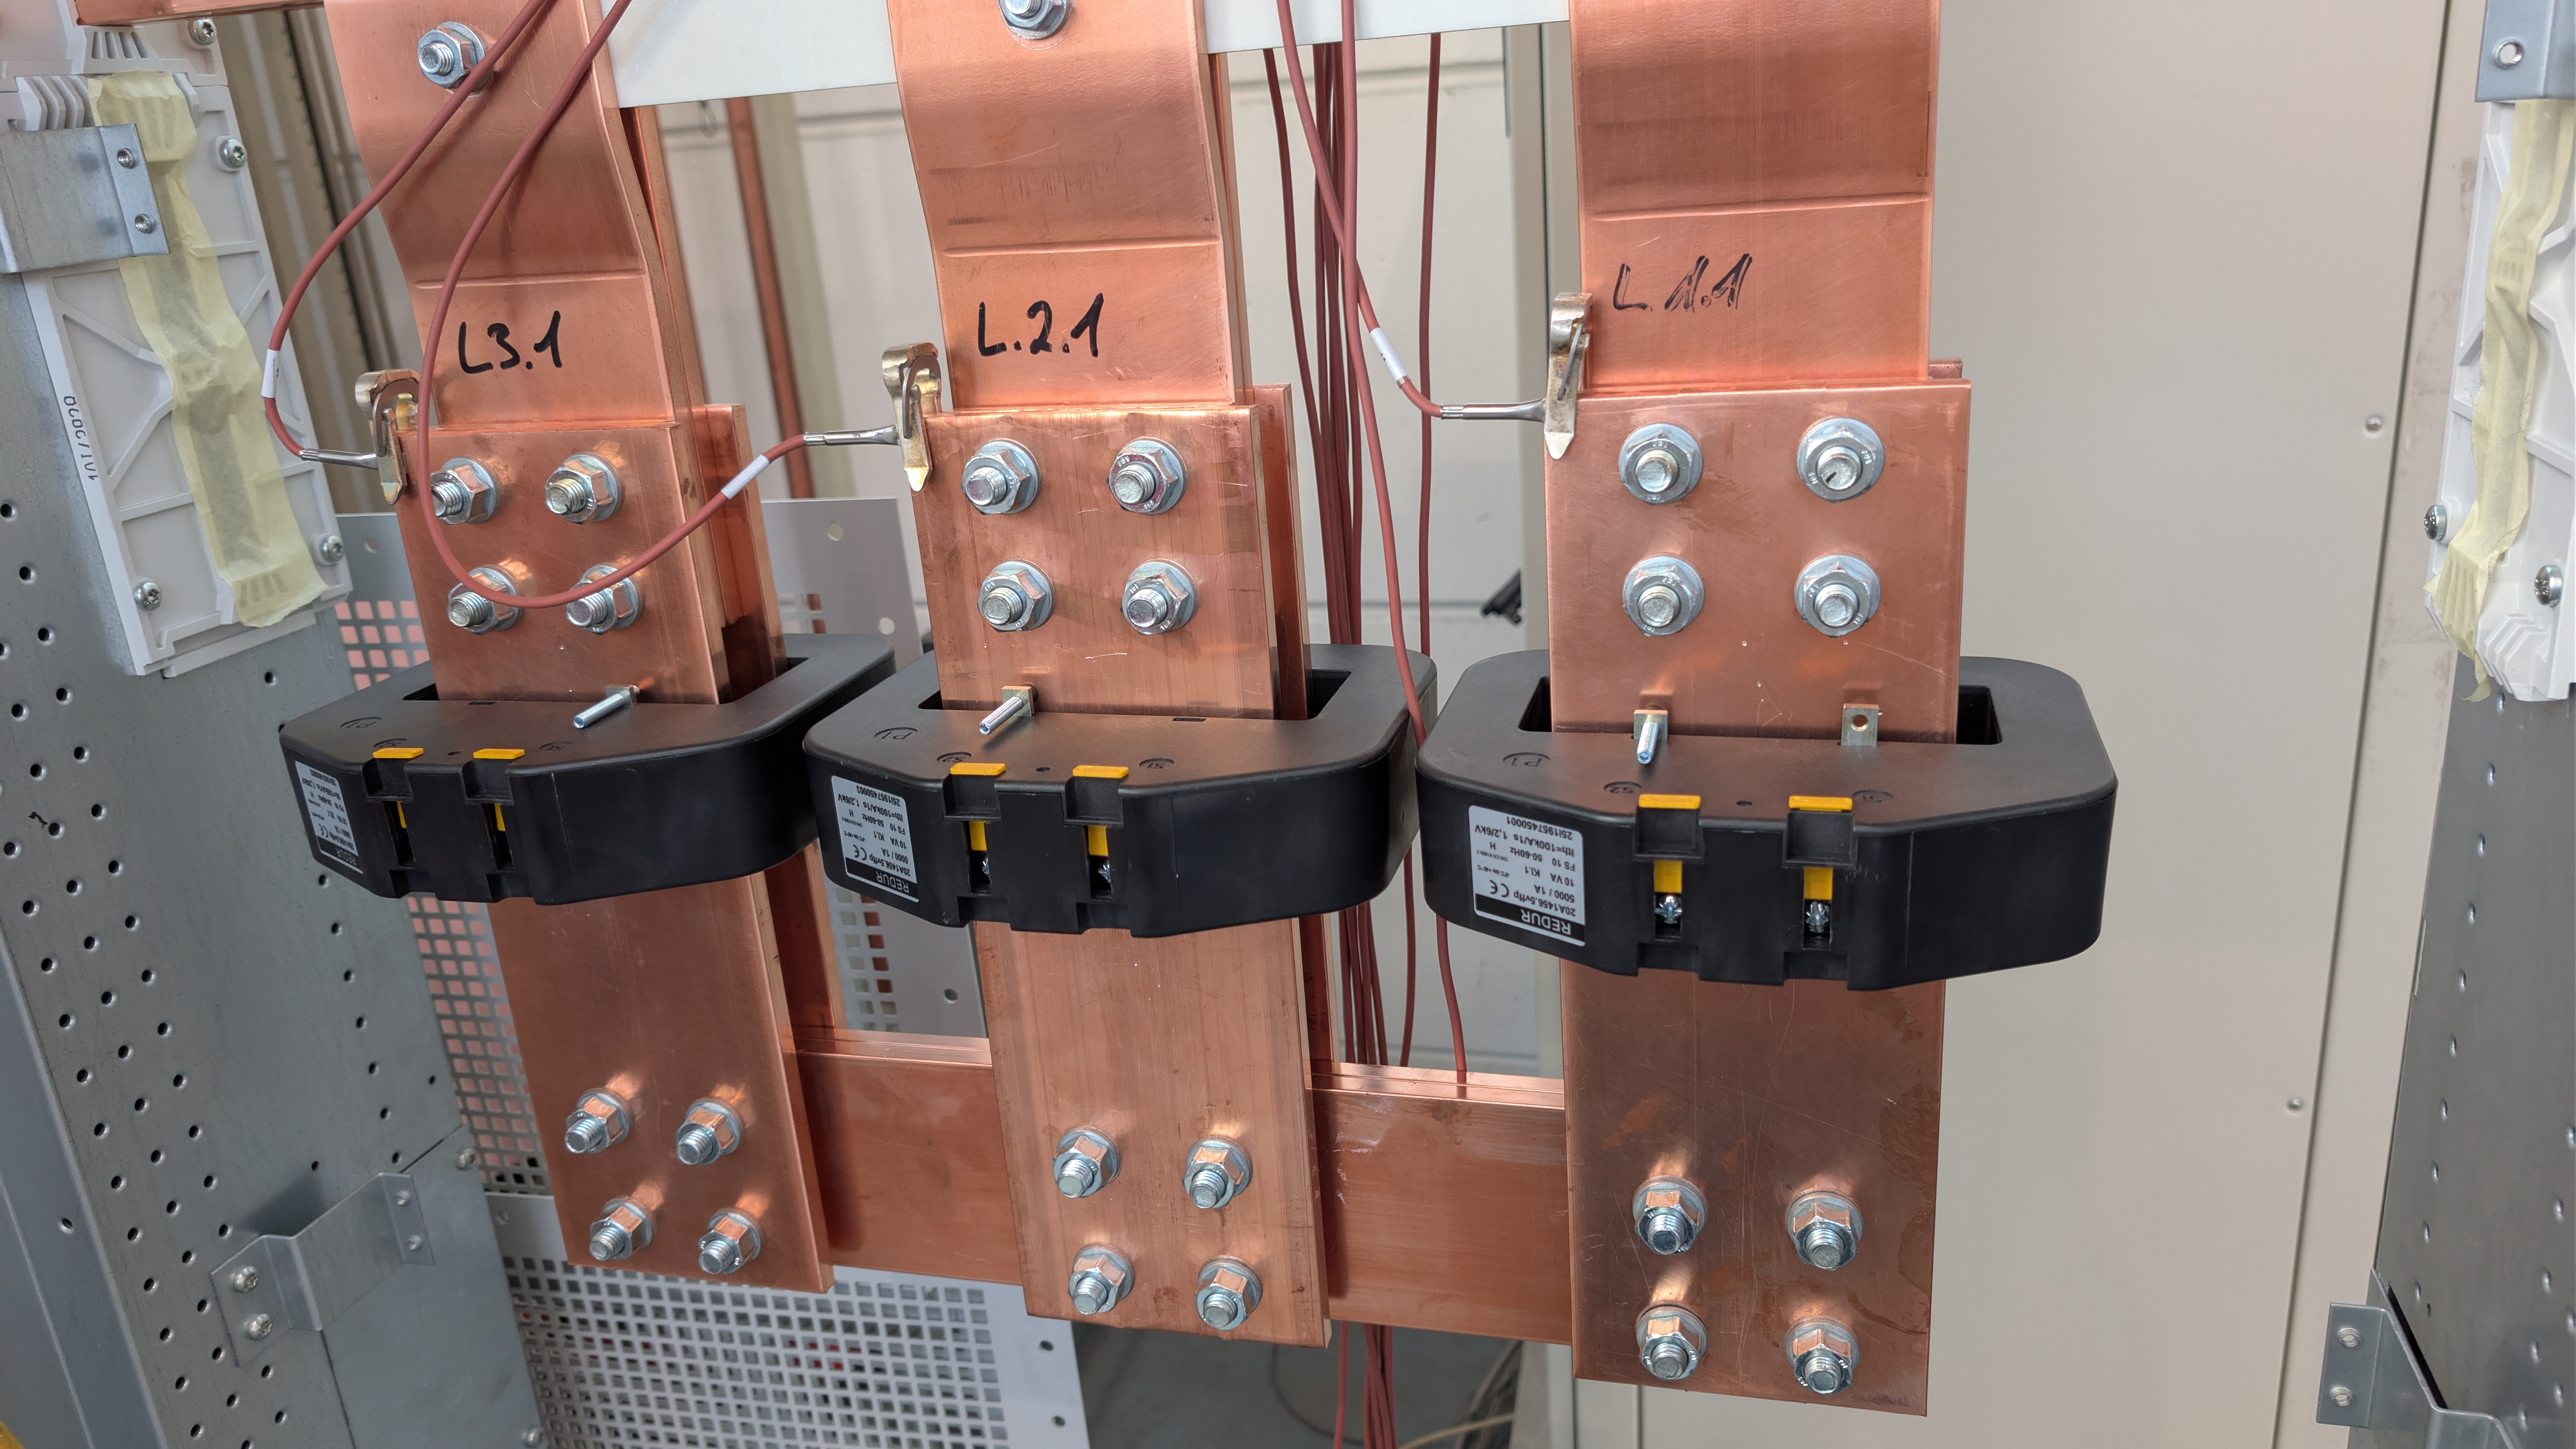
\includegraphics[width=0.8\textwidth]{03_Ressourcen/Bilder/kupferschienen_parallel.jpg}
    \caption{Versuchsaufbau in paralleler Schienenanordnung mit montiertem Messstromwandler (Typ: Redur 20A1456.5vffp)}
    \label{pic:kupferschienen_parallel}
\end{figure}

\textbf{Dreieckskonfiguration}

Zur Realisierung der Dreiecksanordnung wurde ein modifizierter Aufbau entwickelt, der in Abbildung~\ref{pic:kupferschienen_dreieck} dargestellt ist.
Hierbei wird die mittlere Phase (L2) mithilfe eines speziell gefertigten Kupferadapters geometrisch aus der Ebene der Außenleiter herausgeführt.
Der Adapter versetzt die Schiene L2 um \SI{0,1}{mm} nach vorne.

\begin{aufgabenbox}
    Ich muss den Realenabstand noch ermitteltn, wie weit L2 nach vorne verschoben ist.
\end{aufgabenbox}

Durch diesen Versatz spannen die Mittelpunkte der drei Leiter im Querschnitt ein Dreieck auf.
Ziel dieser Anordnung ist es, die magnetische Kopplung zwischen den Phasen symmetrischer zu gestalten und die vektoriellen Anteile der Fremdfelder im Bereich des Wandlerkerns teilweise zu kompensieren.
Auch in dieser Konfiguration wurde der \SI{5000}{A}-Wandler von Redur vermessen.

\begin{figure}[H]
    \centering
    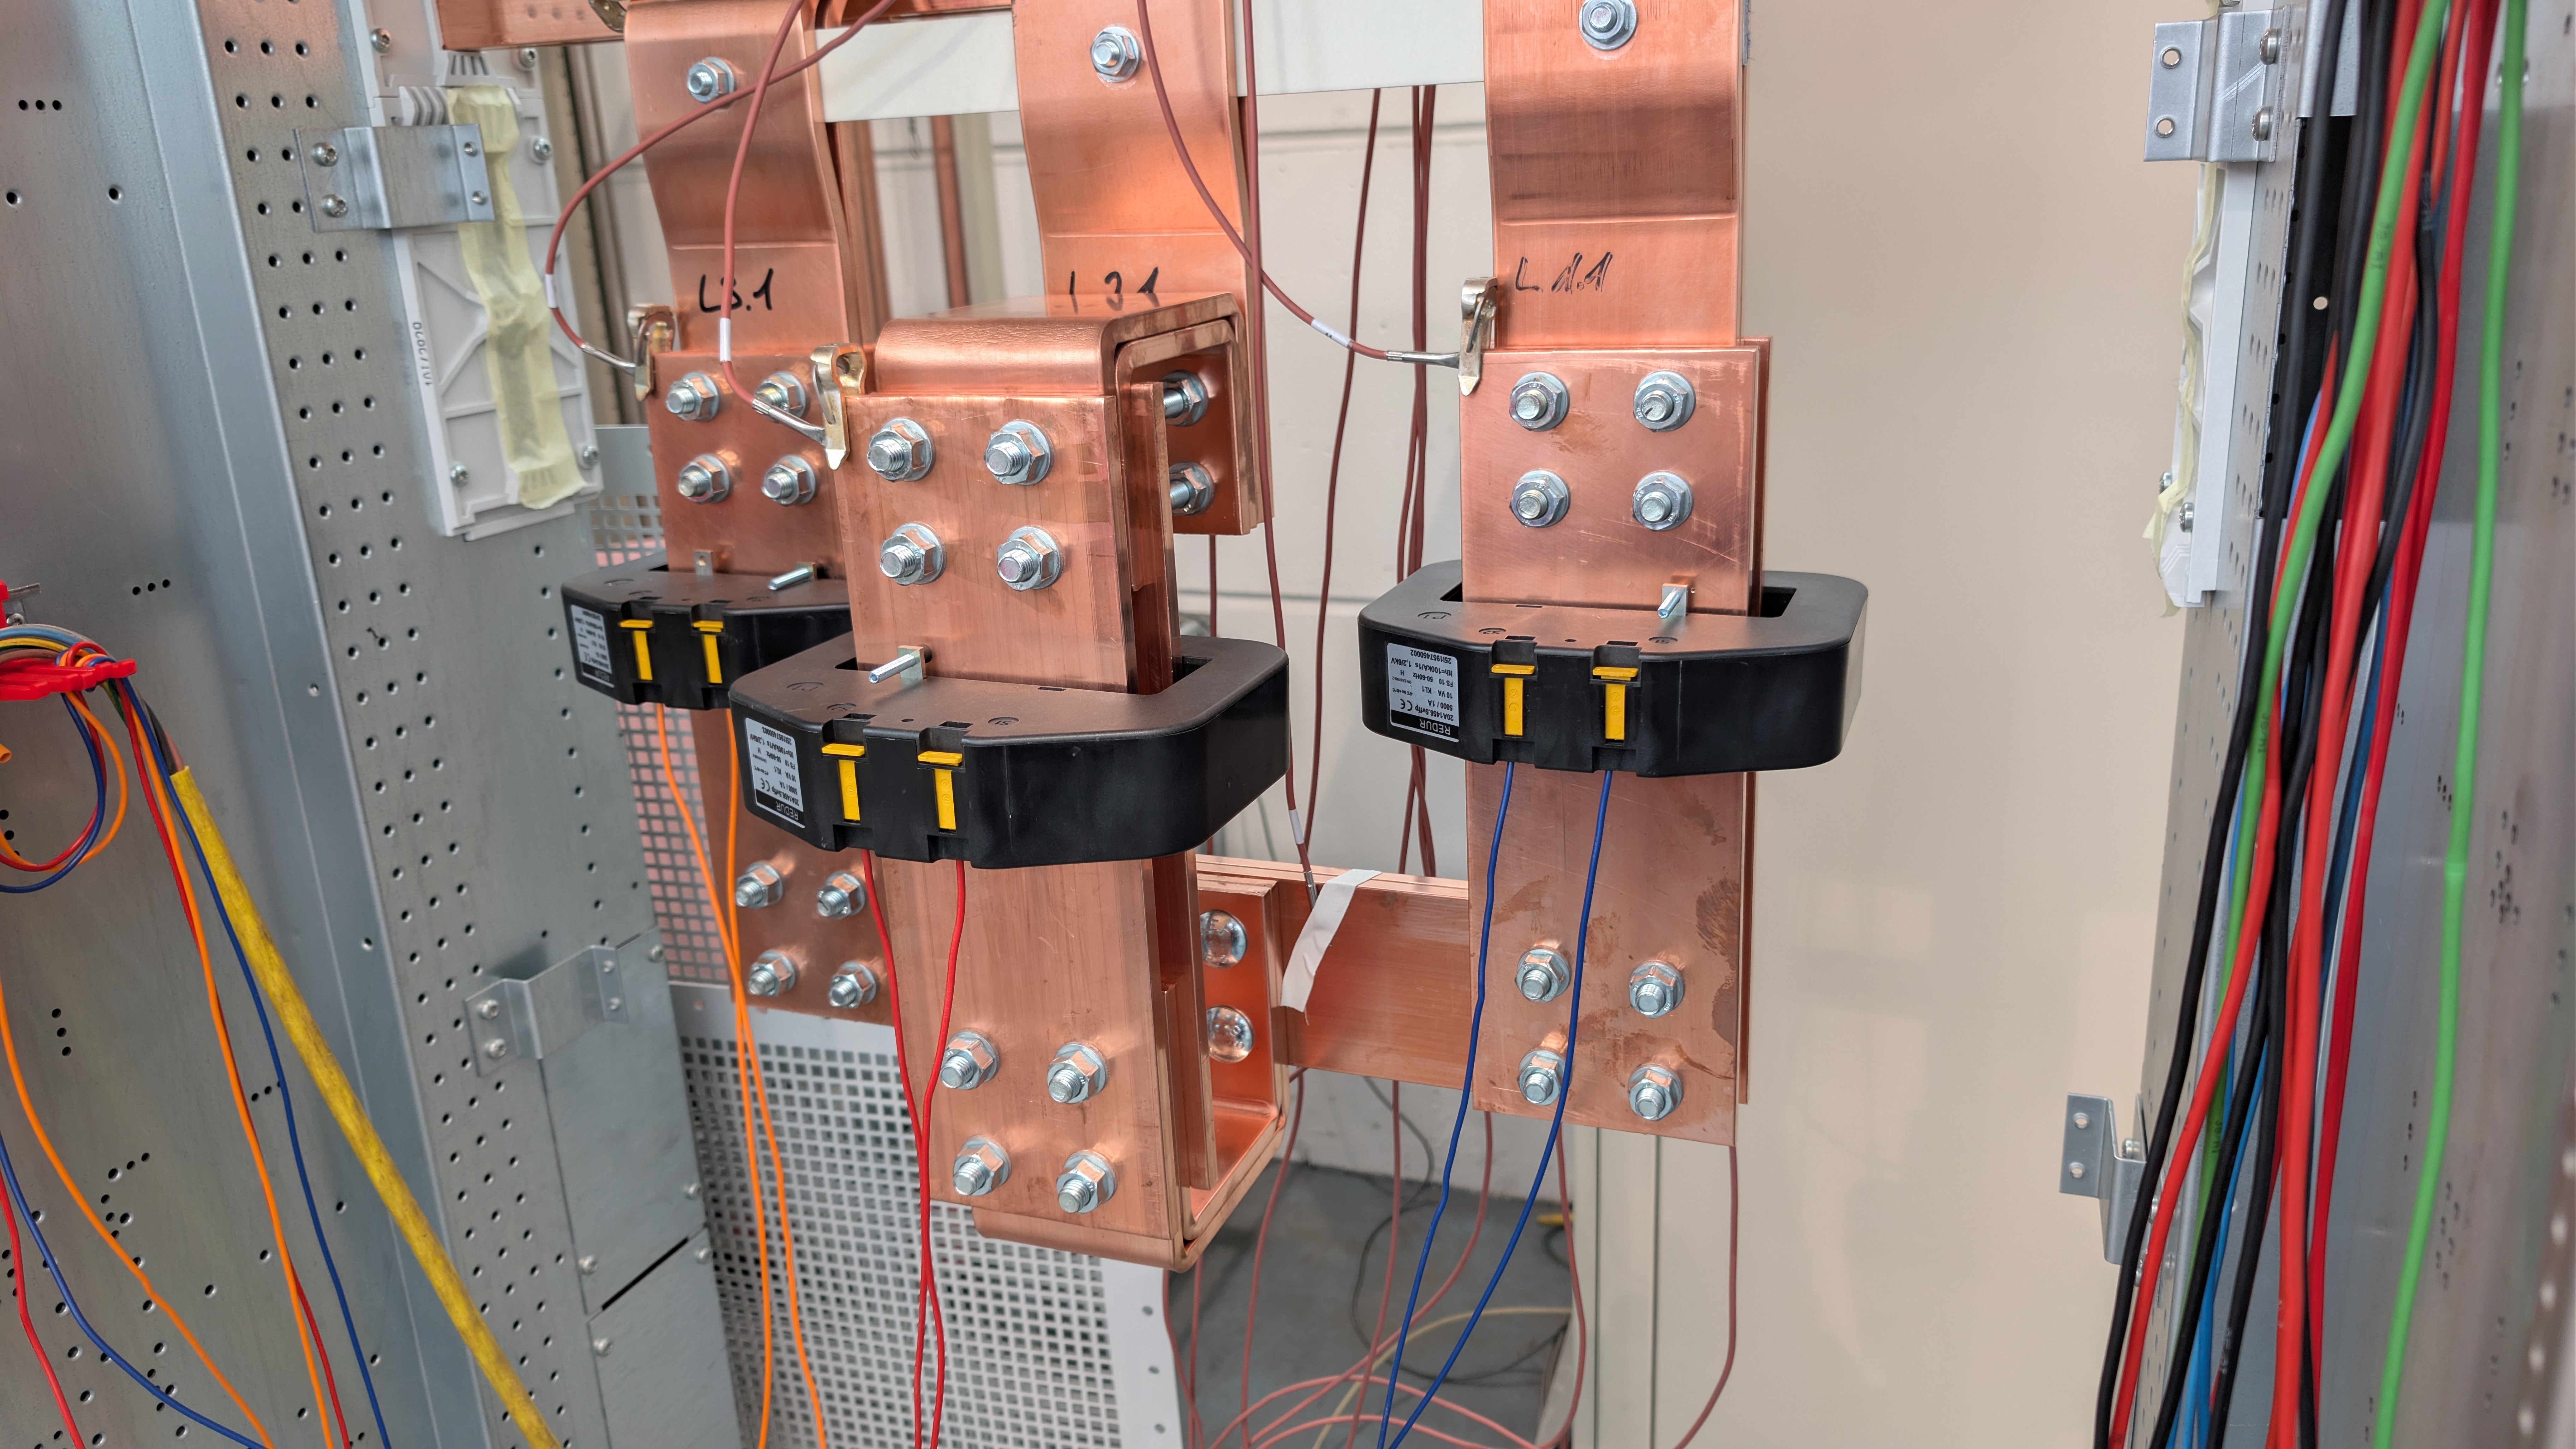
\includegraphics[width=0.8\textwidth]{03_Ressourcen/Bilder/kupferschienen_dreieck.jpg}
    \caption{Modifizierter Versuchsaufbau in Dreieckskonfiguration durch räumlichen Versatz der Phase L2 mittels Kupferadapter}
    \label{pic:kupferschienen_dreieck}
\end{figure}